\ifx\doclanguage\english
\chapter{Technical Background}

This section discusses the background information needed to comprehend the subject and the technologies that are essential to this research. Starting with AgentSpeak(L), which is one of the key use cases for this thesis, we will go through a variety of subjects. Then we switch to Smart contracts built on the \ac{BCT} protocol. The core of this thesis is the creation of supply chain agents and the initiation of their interaction in \ac{BCT} smart contracts, which are thoroughly detailed in this chapter. We go into great depth on the various implementations that enable us to operate Agents with smart contracts. We would next discuss the planning and execution of the key points of this thesis.

\section{Agent}

\subsection{\textit{What is an agent?}}
An \textit{agent} is a reactive system with some autonomy in the sense that if a task is assigned to it, the system determines the optimal way to complete the task. These systems are referred to as "agents" because they are regarded as active, purposeful producers of actions: they are sent out into their environment to achieve objectives, and actively pursue these objectives, figuring out how tasks are to be done for themselves rather than being told in low-level detail how to do so. If they are robotic agents, they may be assigned tasks like as organizing a trip for us, buying tickets to booking hotels, bidding on our behalf in an online auction, and many other tasks that we can conceive of delegating.


\subsection{Characteristics of Agents}

We define agents as systems that exist in a certain context. This means that agents can sense their surroundings (through sensors) and have a repertoire of possible actions to do (via effectors or actuators) in order to affect their surroundings. The essential question for the agent is how to transition from sensor input to action output: how to decide what to do depending on sensor data. An agent's environment can be physical (in the case of robots inhabiting the physical world) or software-based (in the case of a software agent inhabiting a computer operating system or network).

\vspace{.5cm}

Decisions regarding what action to do are turned into real actions by some method external to the agent; often, this is accomplished through some type of \ac{API}. In practically all realistic applications, agents have very limited influence over their surroundings. As a result, while individuals may take acts that alter their surroundings, they cannot entirely control it. This is frequently due to the presence of other agents in the environment who have influence over their portion of the environment. Aside from being located in an environment, the following characteristics are expected of a rational agent:

\begin{itemize}[label={}]
    \descitem{Autonomy}
    At its most basic, autonomy implies being able to work freely in order to attain the goals assigned to an agent. Thus, an autonomous agent, at the very least, makes independent judgments about how to attain its designated goals; its decisions (and thus actions) are under its own control and are not influenced by others.
    
    \descitem{Proactiveness}
    Being proactive entails being able to engage in goal-directed behavior. If an agent has been assigned a specific goal, we expect the agent to make every effort to fulfill that goal. Proactivity eliminates completely passive agents who never strive to accomplish anything. As a result, we don't normally conceive of an object as an agent in the Java sense: such an object is effectively inert until somebody runs a method on it, i.e. instructs it what to do.
    
    \descitem{Reactivity}
    It is not difficult to design a system that merely responds to external stimuli in a reflexive manner; such a system can be constructed as a lookup table, which just translates environment states directly to actions. Similarly, creating a fully goal-driven system is not difficult. (After all, typical computer programs are ultimately just chunks of code designed to fulfill certain goals.) However, putting in place a system that achieves an appropriate mix of goal-directed and reactive behavior is difficult. This is one of the primary design goals of AgentSpeak.
    
    \descitem{Social ability}
    In this context, social ability refers to an agent's ability to collaborate and coordinate actions with other agents in order to achieve goals. To realize this type of social ability, it is necessary to create agents that can interact not just in terms of exchanging bytes or calling procedures on one another, but also at the knowledge level. That is, agents should be able to communicate with one another about their opinions, aims, and plans.
    
\end{itemize}

\subsection{\ac{MAS}}
\textit{'Single agent systems'} are uncommon in practice. The more usual scenario is for agents to coexist in an environment with other agents, resulting in a multi-agent system.
Each agent has the unique capacity to control a portion of its surroundings, but more generically, and more problematically, the domains of influence in the environment may overlap, implying that the environment is jointly controlled by more than on agent. This complicates life for our agents because, in order to accomplish the desired outcome in the environment, our agent must consider how the other agents with some influence are likely to respond.

\vspace{.5cm}

Agents may have different organizational ties to one another; one agent may be a peer to another or have line authority over another. Eventually, these agents will have some awareness of one another, however one agent may not have comprehensive knowledge of the other agents in the system.

\vspace{.5cm}

A language that supports goal-level delegation, support for goal-directed problem solving, lends itself to the creation of systems that are responsive to their environment, should cleanly integrate goal-directed and responsive behavior, and should support knowledge-level communication and cooperation are all necessary for making all the agents in MAS interact with one another.

\section{\ac{BDI} Agent Model}

\subsection{Introduction}

The \ac{BDI} software model is a programming approach for intelligent agents. Although it appears to be defined by the implementation of an agent's beliefs, desires, and intentions, it really employs these notions to address a specific challenge in agent programming \cite{ap}. 

\vspace{.5cm}

In essence, it offers a technique for distinguishing between the action of picking a plan and the execution of already active plans. As a result, \ac{BDI} agents may balance the time spent discussing about plans and implementing those plans. The system designer and programmer are in charge of the third activity, which is planning—making the plans in the first place. This activity is outside the model's purview.

\subsection{Architecture}

This section outlines the \ac{BDI} system's modeled architecture, also shown in Figure \ref{BDI Architecture}.

    \begin{figure}[h]
    \centering
      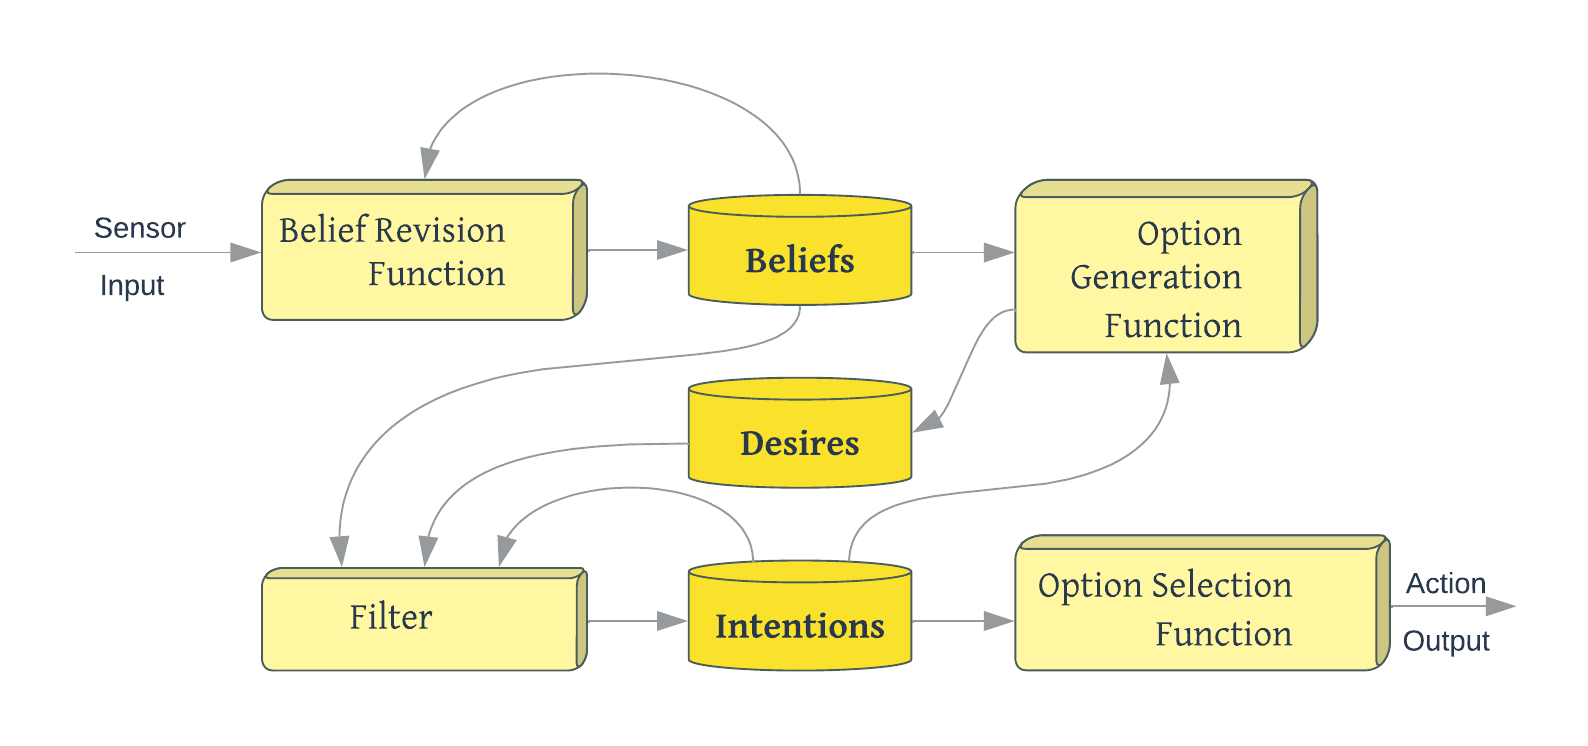
\includegraphics[width=12cm]{includes/figures/BDI_arch.png}
      \caption{\ac{BDI} Architecture}
      \label{BDI Architecture}
    \end{figure}
    
\begin{itemize}
    \descitem{Beliefs} 
    Beliefs reflect the agent's informational state, or its perspective (including itself and other agents). Inference rules can also be included in beliefs, allowing forward chaining to lead to new beliefs. Using the word belief rather than knowledge acknowledges that what an agent believes may or may not be accurate (and in fact may change in the future). One or more belief states and a belief set constitute a belief model.
 
 \vspace{.5cm}
 
    \begin{itemize}[label={}]
        \descitem{Belief set}
        A collection of object diagrams that outline the subject matter of an agent class's beliefs serve as the specification for the belief set. A set of instance diagrams that specify a specific instance of the belief set is referred to as a belief state. Although this is an operational decision, beliefs are maintained in a database (also known as a belief foundation or a belief set).
    \end{itemize}
    
    \vspace{.5cm}
    
    \descitem{Desires}
    Desires indicate the agent's motivational state. They reflect goals or scenarios that the agent wishes to achieve or create.
    
    \vspace{.5cm}
    
    \begin{itemize}[label={}]
        \descitem{Goals}
        A desire that has been embraced for active pursuit by the agent is referred to as a goal. The additional requirement that the collection of active wants must be consistent is added when the term "goals" is used.
    \end{itemize}
    
    \vspace{.5cm}
    
    \descitem{Intentions}
    Intentions depict the agent's deliberate state, or what the agent has decided to do. Intentions are aspirations that the agent has made some commitment to. This indicates that the agent has started carrying out a strategy in implemented systems.
    
    \vspace{.5cm}
    
    \begin{itemize}[label={}]
        \descitem{Plans}
        Plans are collection of instructions that an agent can follow to carry out one or more of its objectives. They can be thought of as recipes or knowledge bases. Plans could incorporate different plans. Three different categories of nodes—start states, end states, and internal states—as well as one kind of directed nape of the neck the plan graph's constituent parts.
        
        \vspace{.5cm}
        
        \begin{itemize}[label={}]
        \descitem{Plan Execution}
        An \textit{activation event} and \textit{activation condition}, which specify when and in what context the plan should be activated, are labeled on the plan graph's first transition. The activation event could be a goal event that happens as a result of the accomplishment of a sub goal activity in another plan, leading to goal-driven activation, or a belief event that happens when an agent's beliefs change or when certain external changes are noticed. If more than one plan is relevant to an event in a particular context, they are either engaged concurrently if the activation is event-driven or progressively until they are successfully terminated if the activation is goal-driven. When a plan is activated, an action may be conducted with the help of an optional activation action.
        
        \vspace{.5cm}
        
        Events pass and fail may be used to indicate the success or failure of the activity connected with the active state during transitions between them. Activities may be halted by transitions from active states that are denoted with the event any whenever their condition is satisfied. The transition of a plan that is aborted is a specific instance of this. The plan fails if the abort condition is true at any point during the execution of its body after it has been triggered. The final transitions of the plan graph may be labeled with the steps to be taken in the event that the plan is successful, unsuccessful, or abandoned.
        
        \vspace{.5cm}
        
        \descitem{Failure}
        The semantics of plan graphs includes the idea of failure. When an action on a transition fails, when there is an explicit transition to a fail state, or when the activity of an active state ends in failure with no outbound transition enabled, failure inside a graph can happen.
        \end{itemize}
    \end{itemize}
    
    \vspace{.5cm}
    
    \descitem{Events}
    In a nutshell, events function as triggers for the agent to react. An event may alter aims, activate plans, or update beliefs. Externally produced events may be picked up by sensors or other connected systems. Events may also be produced internally to start decoupling updates or activity plans.
\end{itemize}

In order to include obligations, norms, and commitments of agents acting within a social context, the \ac{BDI} was further enhanced with an obligations component, giving rise to the \ac{BOID} \cite{boid} agent architecture.


\section{Agent Programming}

In the \ac{AOP} paradigm, the idea of software agents serves as the foundation for the development of the software. \ac{AOP} has externally stated agents (with interfaces and messaging capabilities) at its core as opposed to \ac{OOP}, which has objects (offering methods with variable parameters) at its foundation. They might be viewed as abstractions of actual items. Messages are interpreted in a class-specific manner by receiving "agents."

\subsection{\ac{AOP} versus \ac{OOP}}

\ac{AOP} specialising the framework by fixing the state (now called mental state) of the modules (now called agents) to consist of components such as beliefs (along with beliefs about the world, about themselves, and about one another), capabilities, and decisions, each of which enjoys a precisely defined set of properties. OOP proposes viewing a computational system as being composed of modules that are able to communicate with one another and that have individual ways of handling incoming messages.  Table \ref{AOP versus OOP} summarizes the relation between \ac{AOP} and \ac{OOP}.

\vspace{.5cm}

A variety of restrictions are imposed on an agent's mental state, which generally match to restrictions placed on their common sense equivalents. These agents notify, request, offer, accept, reject, compete, and help one another to do a computation. This concept is directly adapted from the literature on speech acts \cite{speech}. Speech is categorized according to speech acts, which include informing, requesting, offering, and more. Each of these communication acts has a unique set of assumptions and outcomes. \ac{AI}, natural language processing, and plan recognition all use speech act theory.
 Table \ref{AOP versus OOP} summarizes the relation between AOP and OOP

\vspace{.5cm}

\begin{table}[h]
\small
\centering
\caption{\ac{AOP} versus \ac{OOP}}
\label{AOP versus OOP}
\resizebox{11cm}{!}{%
\begin{tabular}{|l| l| l|}
\hline
\textbf{} & \textbf{\ac{AOP} } & \textbf{\ac{OOP}} \\ 
\hline\hline
\textbf{Fundamental Unit} & Agent  &  Object\\ \hline 
\textbf{Parameters defining} & beliefs, commitments,  & Unconstrained\\
\textbf{state of basic unit} &  capabilities, choices .... & \\ \hline 
\textbf{Computation process} & message passing and  &  message passing and \\ 
 & response methods & response methods\\ \hline 
\textbf{Types of message} & inform, request, offer,  & Unconstrained\\ 
 & promise, decline .... & \\ \hline 
\textbf{Constraints on methods} & honesty, consistency ....  &  None\\ 
\hline \hline 
\end{tabular}}
\end{table}

\vspace{.5cm}

\subsection{AgentSpeak(L): \ac{BDI} Agents Interaction}

AgentSpeak(L) is a simplified textual version of \ac{PRS} \cite{prs} or \ac{dMARS} \cite{dmars}. In most ways, the language and its operational semantics are comparable to the implemented system. The implemented system includes extra language constructs to facilitate agent programming.

\vspace{.5cm}

AgentSpeak(L) is a programming language that uses a restricted first-order language with events and actions as its core. The programs created in AgentSpeak(L) govern the agent's behavior (i.e., its interaction with the environment). The agent's beliefs, desires, and intentions are not explicitly stated as modal formulae.

\vspace{.5cm}

The agent's existing belief state may be considered as a model of itself, its environment, and other agents; states that the agent intends to bring about based on external or internal stimuli can be considered as desires; and the adoption of programs to meet such stimuli can be characterized as intentions. This shift in perspective of using a basic specification language as an agent's execution model and then ascribing mental attitudes such as beliefs, desires, and intentions from an external standpoint is more likely to integrate practice and theory.

\subsubsection{Jason}

The agent program and an agent architecture can be differentiate as, the software framework in which an agent program operates is referred to as the agent architecture. The \ac{PRS} is an example of an agent architecture, and the plans are the software that exists within it. We design the program that will drive the agent's behavior, but the architecture itself determines most of what the agent does without the programmer having to worry about it. Jason's language is an extension of AgentSpeak, which is based on the \ac{BDI} architecture. As a result, a belief basis is one of the components of the agent architecture. Another key component is the agent's goals, which are realized through plan execution.

\vspace{.5cm}

It has become customary to include a simple example program to aid comprehension. Hence, an example of Jason AgentSpeak code:

\vspace{.5cm}

\begin{lstlisting}[backgroundcolor = \color{white}, frame=none, numbers=none]
	 started.

    +started <- .print("Hello, I'm an Agent").
\end{lstlisting}

\vspace{.5cm}

Let us attempt to grasp some of what is going on here. The first thing to realize is that this is the definition of a single agent. This specification is generally kept in a single file with the \texttt{'.asl'} extension. Agent's basic beliefs is described in the first line. The full stop, \texttt{'.'}, serves as a syntactic separator in the same way as a semicolon does in Java or C. The next line establishes a plan for the agent, which is the sole plan this agent possesses. This action will display \texttt{'Hello, I'm an Agent'} on the user's terminal. Later, more goals and sub-goals also can be added, according to the plans and requirements.

\subsubsection{\ac{ASTRA}}

\ac{ASTRA} is also based on AgentSpeak(L) in that it provides all of the same fundamental capabilities as AgentSpeak(L), but it also adds a number of extra features that makes it more practical Agent Programming Language. The fundamental distinction between beliefs, aims, and events is that words and variables are typed. \ac{ASTRA}'s type system is based on the Java type system, mainly because Java is the underlying implementation language, and using a comparable type system makes translating between \ac{ASTRA} and Java easier and more visible.

\vspace{.5cm}
As a result, \ac{ASTRA} programs are more organized than AgentSpeak(L) applications. The basic structure is seen below:

\vspace{.5cm}

\begin{lstlisting}[backgroundcolor = \color{white}, frame=none, numbers=none]
     package path.to.folder;
     import java.lang.Object;
     
     agent Hello {
         module Console console;
    
         initial !init();
    
         rule +!init() {
             console.println("Hello, I'm an Agent");
         }
     }
\end{lstlisting}

\vspace{.5cm}

As can be observed, \ac{ASTRA} has embraced the Java \texttt{package} and \texttt{import} nomenclature. The \texttt{agent} keyword denotes the beginning of the agent program, and curly braces represent the body of that program (known here as an \texttt{agent class}). This specification is generally kept in a single file with the \texttt{'.astra'} extension. This action will also display \texttt{'Hello, I'm an Agent'} on the user's console.

\section{Web3}

\subsection{Background}
The terms "Web 1.0" and "Web 2.0" refer to phases in the development of the World Wide Web using different technology and formats. Web 1.0 refers to a time when the bulk of websites just had static pages and the great majority of people consumed information rather than created it. Web 2.0 is centered on user-generated content that is published to forums, social media and networking sites, blogs, and wikis, among other services. It is founded on the concept of "the web as platform."

\subsection{Introduction}
An notion for a new version of the World Wide Web called Web3 (sometimes referred to as Web 3.0) integrates ideas including decentralization, blockchain technology, and token-based economy. Some journalists and engineers have compared it to Web 2.0, where they claim that content and data are concentrated in a select few businesses frequently referred to as "Big Tech."

\vspace{.5cm}

Web3's specific goals vary, and the phrase has been characterized as "ambiguous," but they all revolve on the concept of decentralization and frequently include \ac{BCT}, including multiple crypto-currencies and \ac{NFT}. The concept of Web3 would include financial resources, in the form of tokens. It can alternatively be described as the ostensible next generation of the web's technological, legal, and monetary infrastructure, which includes crypto-currencies, blockchain, and smart contracts. Web3's three core architectural enablers were recognized as a mix of decentralized or federated platforms, safe interoperability, and verifiable computing via distributed ledger technologies.

\vspace{.5cm}

The idea of \ac{DAO} serves as the foundation for several concepts. On addition to owning your data in Web3, you can also use tokens that function like stock to collectively own the platform. \ac{DAO} enables decentralized platform ownership coordination and future platform decision-making. Another important idea is \ac{DeFi}, which allows for money exchange without the intervention of banks or the government. \ac{SSI} enables users to identify themselves without depending on an authentication system like OAuth \cite{oauth}, where identity verification requires contacting a trusted party. Web3 would most likely coexist with Web 2.0 websites, with Web 2.0 websites most likely adopting Web3 technology to keep their services updated.

\subsection{Concept}

Web 3.0 may be recognized by a collection of traits that are altering how people connect outside of the physical world and have an impact on how businesses are made: 
\begin{itemize}

    \item  Individualized - Information may be divided into context-relevant segments based on network contacts and personal preferences. In fact, one of the features of Web 3.0 is the capacity to deal with unstructured content on the Web more intelligently by giving the published data about individual or group factors contextual meaning. The social networks are a well-known method of connection with a very broad audience of adopters. People may choose their own exposure and contacts depending on information preferences and "proximity".

    \item 
  Ubiquity - People can connect at any time and from any location. Staying connected is made easier by a variety of communication alternatives, including mobile networks, Wi-Fi networks, cable networks, or cellular networks, as well as many device kinds, including laptops, desktop computers, tablets, and an endless array of mobile devices. Regardless of the architectures or systems being used


    \item  Efficient - Both people and computing devices are capable of filtering information based on context, meaning, and relevance. This trait has an implied connection to the individualized trait. Regarding individual variances, knowledge causes various responses in various persons. The capacity to filter content based on user interests appears to be a benefit of Web 3.0. Efficiency requires that the information must be organized such that algorithms can read it and comprehend it as clearly and completely as humans can.

\end{itemize}
\section{Blockchain}

\subsection{Introduction}
Blockchain is a decentralized ledger system that may be used to store data across numerous cluster nodes. A typical blockchain network's cluster of nodes cannot be controlled by a single organization, hence the system is decentralized. The blockchain data is computationally authenticated by the majority of unconnected nodes in a cluster of arbitrary 'N' nodes. This fundamental architecture of blockchain assures that it is not controlled by a centralized authority and that the system as a whole is 'trustless.' We imply that there is no need to trust the source of data or the provider since mathematical computations and decentralized validation make the system computationally trustworthy.

\vspace{.5cm}

Due to the lack of a single administrator who has access to change and remove the recorded data, this feature of blockchain technology assures that the data has not been altered. It displays characteristics like immutability, irrevocability, and non-repudiation as a result of its construction. Due to these characteristics, it is the perfect answer for several significant real-world use cases, including financial applications.

\vspace{.5cm}

The modern blockchains allow users to create their own custom code that is then performed as functions inside the ecosystem and the outputs of these functions are added to the blockchain's updated state. These functions are often run at numerous network nodes and a consensus on the status of outcomes is reached. These tasks or workloads are known as smart contracts in Ethereum and several other public blockchains, and chaincodes in Hyperledger Fabric.


\subsection{Architecture}
According to its technical definition, a blockchain is a series of interconnected blocks that, as seen in Figure \ref{Blocks chained together in a blockchain}, include the data on a group of transactions up to the most recent block. The block headers retain the details of their own hash, that of their preceding block, a list of transactions, and the time stamp. In the blockchain network, these characteristics are utilized to track a specific transaction. All blockchain nodes save a block as the most recent state once it has been approved and confirmed by the majority of network participants.

 \vspace{.5cm}
 
\begin{figure}[h]
  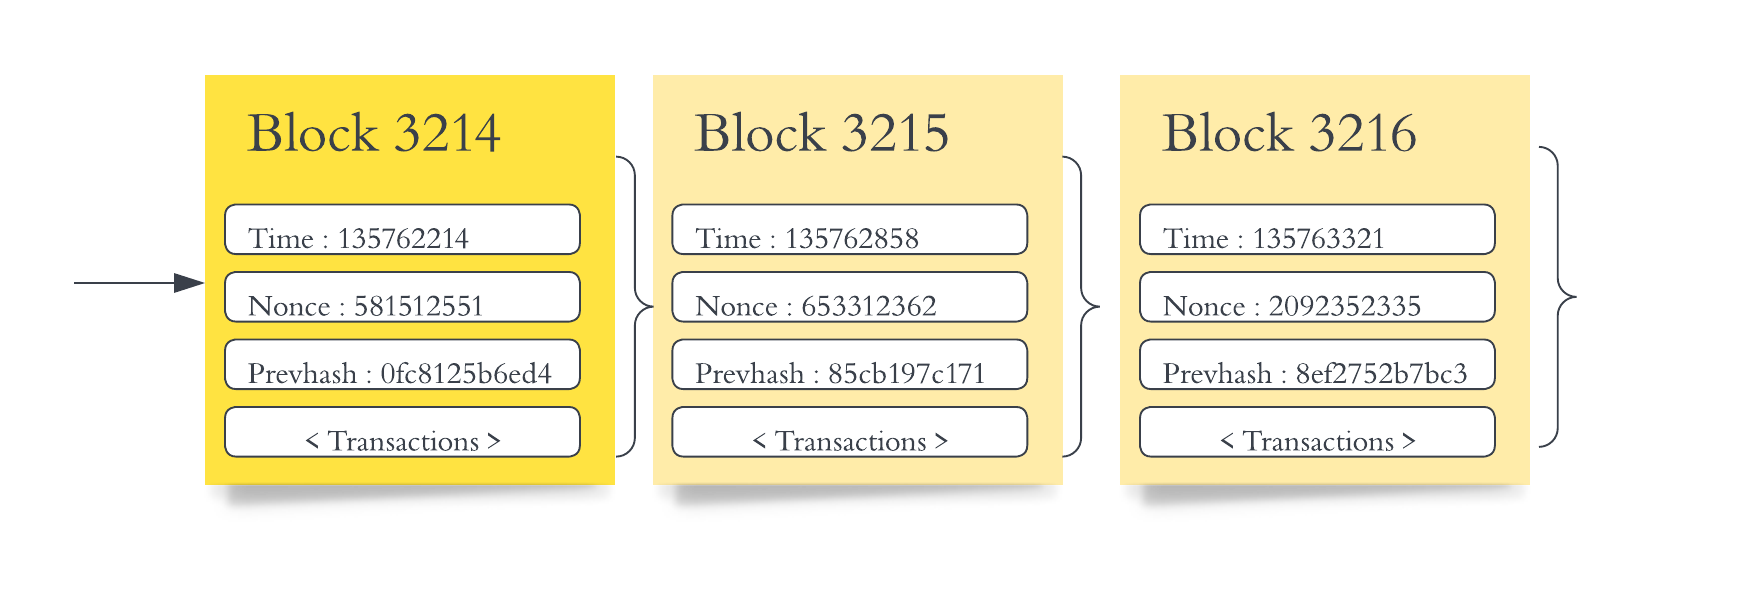
\includegraphics[width=\textwidth]{includes/figures/blocks.png}
  \caption{Blocks chained together in a blockchain}
  \label{Blocks chained together in a blockchain}
\end{figure}

 \vspace{.5cm}
 
Different procedures, including as \ac{PoW} \cite{pow}, \ac{PoS} \cite{pos}, and \ac{PoA} \cite{poa}, etc., are available to reach agreement on the choice of a block.
 
\vspace{.5cm}
 
On a higher level, blockchains may be split into two categories: permissioned and permissionless. Consortial and private blockchains are also included in the permissioned blockchains, whereas public blockchains are included in the permissionless blockchains. Below, we explore these categories' characteristics.

\subsubsection{Public Blockchains}

Public blockchains are permission-less blockchains in which anybody with a personal computer may run an open-source protocol and connect to the network as an equal node. The public blockchains run completely decentralized peer-to-peer systems. They are the perfect approach for implementing digital currency. The most well-known public blockchains are Ethereum and Bitcoin.

\subsubsection{Private Blockchains}

Private blockchains are distributed node clusters that operate within a secure private network and store and process data according to blockchain rules. Private blockchains are governed by a centralized organization rather than being decentralized in nature. They primarily serve as a distributed ledger that is scalable. Private blockchains often employ the lightweight \ac{PoA} protocol to add new blocks.

\subsubsection{Consortial Blockchains}

Consortial blockchains are permissioned blockchains, just as private blockchains, and the general public cannot join them. They belong to a group of priveleged individuals who could be associated with this network. The cluster of nodes is dispersed throughout the intranets of the participating organizations. They are especially helpful when two mutually trusted parties wish to use the distributed ledger's privacy-preserving features. Hyperledger Fabric, Hyperledger Indy, and other consortium blockchains are the most well-known.


\subsection{Smart Contracts}

To begin, we will define smart contracts. Szabo's \cite{def1} definition is as follows:

\vspace{.5cm}

\begin{definition}
  A smart contract is a set of promises, specified in a digital form, including protocols within which the parties perform on these promises.
\end{definition}

\vspace{.5cm}

In order to automatically execute, control, or document legally significant events and activities in accordance with the provisions of a contract or an agreement, a smart contract is a computer program or transaction protocol. The goals of smart contracts are to decrease the need for trustworthy intermediaries, arbitration fees, fraud losses, and malicious and unintentional exceptions. The smart contracts provided by Ethereum are widely regarded as a crucial building block for \ac{DeFi} and \ac{NFT} applications. Smart contracts are frequently linked to cryptocurrencies.

\vspace{.5cm}

A smart legal contract, as opposed to a smart contract, is a conventional, legally-binding pact with specific provisions defined and put into machine-readable code. Smart legal contracts should not be confused with smart contracts.

\subsection{\ac{EVM}}

The second-largest blockchain system in the world is believed to be Ethereum. With smart contracts, Ethereum enhances the blockchain paradigm. The applications running on the Ethereum blockchain are known as smart contracts. Ethereum provides the \ac{EVM} to parse the source code of the contracts into an opcode sequence that is predefined by Ethereum in order to execute the smart contracts. For the Ethereum blockchain to correctly execute contracts and handle transactions, each node requires an \ac{EVM}.

\vspace{.5cm}

The \ac{EVM} may be conceptualized practically as a vast, decentralized system with large numbers of objects, called \textit{accounts}, that can maintain an internal database, run code, and communicate with one another.

\subsection{Solidity: Build Smart Contracts}

The Ethereum blockchain's popularity and disruptive power are directly related to its capacity to execute smart contracts. \ac{BCT} may be effectively used to create \ac{Dapp} using Ethereum platform. A \ac{Dapp} is a tool used to connect individuals and groups on various sides of an interaction without the usage of a centralized intermediary.

\vspace{.5cm}

\textit{Solidity}, a Javascript-like language designed expressly for creating smart contracts, is the primary language used in Ethereum. Among its other characteristics, Solidity is statically typed and enables complicated user-defined types, libraries, and inheritance. The solidity compiler converts source code into \ac{EVM} bytecode so that it may be deployed into the Ethereum network. The owner of the contract is responsible for paying the additional transaction fees associated with contract deployments and smart contract interactions in the form of \textit{gas}.

\subsection{Truffle Suite}
\subsubsection{Truffle}

As a programming environment, testing framework, and asset pipeline for blockchains running on the \ac{EVM}, truffle basically aims to simplify the workload of a developer. Truffle offers built-in binary management, deployment, linking, compilation, and testing for smart contracts in addition to automated contract testing for quick development. It offers configurable build pipeline with support for tight integration, as well as pNPM ackage management using \ac{NPM} and the ERC190 standard, i.e. \ac{ERC}.

\vspace{.5cm}

Truffle supports transactions and deployments with MetaMask to safeguard your mnemonic, which is a pattern of letters, and it offers enhanced debugging with breakpoints, variable analysis, and step functionality.
With an interactive terminal for direct contract communication, it is an external script runner that runs scripts inside the Truffle environment.
Provides a scriptable, extendable framework for deployment and migrations, as well as network management for deploying to any number of public and private networks.

\subsubsection{Ganache}

Ganache is a private blockchain enabling speedy production of Corda and Ethereum distributed applications. Ganache may be used throughout the whole development cycle, allowing you to create, distribute, and test \ac{Dapp} in a secure and predictable setting.

\vspace{.5cm}

Both a \ac{UI} and a \ac{CLI} are available with ganache. A desktop program called Ganache \ac{UI} supports both Corda and Ethereum. Ethereum programming is possible using the powerful command-line tool ganache. It supports snapshot/revert state, Ethereum JSON-RPC compatibility, Zero-config Mainnet and testnet forking, console-log in Solidity, and the ability to impersonate any account without the need for private keys.

\subsection{Vision}
As blockchain technology continues to develop, a number of new blockchains have recently come to light, each with a unique architecture and implementation that has been carefully chosen for the intended use case. Additionally, there are significant flaws in the conventional blockchain architecture that remain unresolved, and other implementations aim to address these concerns. (1) Lack of anonymity in transaction execution (2) High transactional delay owing to complex consensus procedures that cause scalability concerns are the two main outstanding challenges with blockchains. (3) Communication between several blockchains; (4) Integration with the outside world.

\vspace{.5cm}

Each of the more recent blockchain implementations, including Zcash, Polkadot, Ethereum 2.0, Chainlink, etc., is working to find a solution to these problems. With the use of trustworthy execution environments, we also hope to address the aforementioned issues with conventional blockchains in this thesis. Because the burden from the blockchain is transferred to secure execution environments, the blockchains are lightweight and offer transaction execution privacy. In addition, the Hyperledger Avalon has developed blockchain connectors for a number of distinct blockchains that may be used to promote interoperability between them. The Avalon infrastructure may also be used to build "attested oracles," which connect blockchains with data from the outside world.

\section{Jython}

Jython is a Python programming language implementation meant to operate on the Java platform. JPython was the previous name for the implementation. Any Java class may be imported and used by Jython apps. Jython applications, with the exception of a few common modules, employ Java classes rather than Python modules. 

\vspace{.5cm}
Jython provides practically all of the modules found in the standard Python programming language package, with the exception of a few modules written in C. Jython either dynamically or statically converts Python source code to Java bytecode (an intermediate language). The following tasks are especially well suited for Jython:

\begin{itemize}
    \item In order to interact with Java packages or run Java programs, Jython provides an interactive interpreter. This makes it possible for developers to experiment with and debug any Java system using Jython.

    \item Users can write simple or intricate scripts using embedded scripting to increase an application's capabilities. The Jython libraries are available to Java programmers for their systems.

     \item Python scripts are frequently 2–10 times shorter than their Java equivalents, enabling quick development of applications. This has a direct impact on how efficiently programmers work. Python and Java get along well with one another, allowing programmers to mix the two languages at will during both product development and release.
\end{itemize}

